\documentclass[11pt]{article}
\usepackage[margin=1in]{geometry}
\usepackage{amsmath,amssymb}
\usepackage{booktabs}
\usepackage{siunitx}
\usepackage{hyperref}
\usepackage{graphicx}
\usepackage{epstopdf}
\usepackage{caption}
\usepackage{xcolor}
\usepackage{array}

\sisetup{
  separate-uncertainty = true,
  per-mode = symbol,
}

\title{R3: Longitudinal Beam Dynamics and Bunch Compression\\
  for the 0.5\,ps and 2\,ps Operating Modes}
\author{Eremey Valetov}
\date{4 March 2026}

\graphicspath{{../../../../backend/test/}}

\begin{document}
\maketitle

\section{Introduction}

The UH MkV FEL is designed to operate at two bunch lengths: \SI{2}{ps}
(baseline) and \SI{0.5}{ps} (short-pulse mode).  A reviewer asks whether
the transverse matching changes between modes and whether the transport
line can compress a \SI{2}{ps} beam to \SI{0.5}{ps}.

This report consolidates the longitudinal studies (W9, W12) into a
single document.  We extract the full 6D transfer map from
COSY~INFINITY, propagate bunches at both operating modes, test
$R_{56} = 0$ as an optimisation objective, evaluate in-line bunch
compression through chirp, and validate against RF-Track particle
tracking.


\section{Transfer Map Analysis}

\subsection{COSY 6D Map Extraction}

The 11-stage COSY FIT optimisation ($E = \SI{40}{MeV}$,
$\varepsilon_n = 8\;\pi\cdot\text{mm}\cdot\text{mrad}$, FR\,0,
order~3) produces MSE~$= 2.27 \times 10^{-7}$.  The full $6\times6$
linear transfer map $\mathcal{M}$ and the second-order coefficient
$(l|\delta\delta) = \text{ME}(5,66)$ are extracted via the COSY
\texttt{PM} command.

COSY uses $\delta = \delta_K = \Delta K/K_0$ (kinetic energy
deviation).  The standard-optics conversion factor is
$p_0 c / K_0 = 40.508/40 = 1.013$ for \SI{40}{MeV} electrons.

Table~\ref{tab:map} lists the longitudinal map elements at the
undulator entrance.

\begin{table}[ht]
\centering
\caption{Longitudinal elements of the COSY transfer map $\mathcal{M}$ at
  the undulator entrance.  COSY notation $(y_i|y_j)$; transport-code
  equivalents ($R_{ij}$, $T_{ijk}$) for reference.}
\label{tab:map}
\begin{tabular}{@{} l l l S[table-format=+1.4e-1] l @{}}
\toprule
{Map element} & {FOX} & {Transport} & {Value} & {Interpretation} \\
\midrule
$(l|x)$        & ME(5,1)  & $R_{51}$  &  9.874e-3  & Path length from $x$ (dipoles) \\
$(l|a)$        & ME(5,2)  & $R_{52}$  & -4.799e-2  & Path length from $x'$ (dipoles) \\
$(l|y)$        & ME(5,3)  & $R_{53}$  &  0         & Path length from $y$ \\
$(l|b)$        & ME(5,4)  & $R_{54}$  &  0         & Path length from $y'$ \\
$(l|l)$        & ME(5,5)  & $R_{55}$  &  1.000     & Path length identity \\
$(l|\delta)$   & ME(5,6)  & $R_{56}$  &  2.709e-2  & Momentum compaction (\SI{27.09}{mm}) \\
\midrule
$(\delta|x)$   & ME(6,1) & $R_{61}$  &  0         & Energy from $x$ \\
$(\delta|a)$   & ME(6,2) & $R_{62}$  &  0         & Energy from $x'$ \\
$(\delta|\delta)$ & ME(6,6) & $R_{66}$ & 1.000    & Energy identity (implicit) \\
\midrule
$(l|\delta\delta)$ & ME(5,66) & $T_{566}$ & 0     & 2nd-order momentum compaction \\
\bottomrule
\end{tabular}
\end{table}

The transfer map has the expected block structure:
\begin{itemize}
  \item $(\delta|x_j) = 0$ for all transverse $x_j$: no
    transverse$\to$energy coupling.  The transverse and longitudinal
    subspaces are decoupled in the Twiss matching sense.
  \item $(l|x)$, $(l|a) \neq 0$: off-axis particles travel different
    path lengths through dipoles.  This is a geometric effect that
    does not affect transverse matching.
  \item $(l|\delta) = \SI{27.09}{mm}$: the chromatic path-length
    spread converts energy spread into bunch lengthening.
  \item $(l|\delta\delta) = 0$: no nonlinear compression or
    decompression effect.
\end{itemize}


\section{6D Bunch Propagation}

Gaussian bunches ($N = 10{,}000$, seed = 42) are propagated through
the COSY map for four scenarios: 0.5\,ps and 2\,ps, each with
$h = 0$ and $h = 5 \times 10^9$\,s$^{-1}$.

Table~\ref{tab:bunch} summarises the beam parameters before and
after transport.  Table~\ref{tab:emittance} shows the transverse
emittance evolution.

\begin{table}[ht]
\centering
\caption{6D bunch propagation results ($N = 10{,}000$).
  $\sigma_\delta$ is preserved exactly ($(\delta|x_j) = 0$).  Bunch
  length grows due to $(l|\delta) \times \sigma_\delta$ chromatic
  path-length spread.}
\label{tab:bunch}
{\small
\begin{tabular}{@{} l SS SS S @{}}
\toprule
{Scenario} & {$\sigma_z^\text{in}$ ($\mu$m)} & {$\sigma_z^\text{out}$ ($\mu$m)}
  & {$\sigma_\delta^\text{in}$ (\%)} & {$\sigma_\delta^\text{out}$ (\%)}
  & {$\sigma_z$ ratio} \\
\midrule
0.5\,ps, $h{=}0$     & 149.1 & 201.2 & 0.500 & 0.500 & 1.350 \\
0.5\,ps, $h{=}5\text{e}9$ & 149.1 & 255.0 & 0.557 & 0.557 & 1.710 \\
2\,ps, $h{=}0$       & 596.4 & 611.1 & 0.500 & 0.500 & 1.025 \\
2\,ps, $h{=}5\text{e}9$   & 596.4 & 875.8 & 1.111 & 1.111 & 1.469 \\
\bottomrule
\end{tabular}
}
\end{table}

\begin{table}[ht]
\centering
\caption{Transverse emittance through the COSY map.  Horizontal
  projected emittance grows due to $(x|\delta) \times \sigma_\delta$
  chromatic dispersion; vertical emittance is preserved exactly.}
\label{tab:emittance}
{\small
\begin{tabular}{@{} l SS SS @{}}
\toprule
{Scenario}
  & {$\varepsilon_{x,n}^\text{in}$ ($\mu$m)} & {$\varepsilon_{x,n}^\text{out}$ ($\mu$m)}
  & {$\varepsilon_{y,n}^\text{in}$ ($\mu$m)} & {$\varepsilon_{y,n}^\text{out}$ ($\mu$m)} \\
\midrule
0.5\,ps, $h{=}0$     & 8.07 & 9.04 & 8.07 & 8.07 \\
0.5\,ps, $h{=}5\text{e}9$ & 8.07 & 9.26 & 8.07 & 8.07 \\
2\,ps, $h{=}0$       & 8.07 & 9.04 & 8.07 & 8.07 \\
2\,ps, $h{=}5\text{e}9$   & 8.07 & 12.05 & 8.07 & 8.07 \\
\bottomrule
\end{tabular}
}
\end{table}

The 0.5\,ps beam experiences 35\% bunch lengthening ($\to$\SI{0.67}{ps});
the 2\,ps beam is relatively unaffected (2.5\% growth).  The absolute
chromatic contribution ($R_{56} \sigma_\delta = 27.09\;\text{mm}
\times 0.005 = \SI{135}{\micro m}$) is the same for both, but it
represents a larger fraction of the shorter initial $\sigma_z$.
Energy spread is preserved exactly in all cases.

Figures~\ref{fig:phase-space} and~\ref{fig:histograms} show the
longitudinal phase space and bunch profiles.


\section{$R_{56} = 0$ Objective Test}

Table~\ref{tab:r56obj} compares the baseline (transverse-only) and
augmented ($+ (l|\delta) = 0$) COSY FIT results.

\begin{table}[ht]
\centering
\caption{Effect of adding $(l|\delta) = 0$ as a COSY FIT objective.
  The optimiser produces identical results.}
\label{tab:r56obj}
\begin{tabular}{@{} l S[scientific-notation=true] S[table-format=2.4] S[table-format=1.6] @{}}
\toprule
{Configuration} & {MSE} & {$(l|\delta)$ (mm)} & {Max $|\Delta I|$ (A)} \\
\midrule
Transverse only   & 2.27e-07 & 27.0890 & {---} \\
Transverse + $(l|\delta){=}0$ & 2.27e-07 & 27.0890 & 0.000000 \\
\bottomrule
\end{tabular}
\end{table}

Adding $(l|\delta) = 0$ has zero effect: identical solution, identical
currents, identical $R_{56}$.  Verification with extreme weights
($w = 100$ and $w = 10{,}000$) confirms that the Stage~11 quadrupoles
have negligible leverage over $R_{56}$: at $w = 10{,}000$, the best
reduction is only \SI{9}{\micro m} (0.03\%) while transverse MSE
degrades by $2300\times$.  The $R_{56}$ is geometry-locked by the
dipole angles and spacings.


\section{Bunch Compression Feasibility}

\subsection{Analytical Framework}

With linear chirp $h$ (s$^{-1}$) and momentum compaction $R_{56}$:
\begin{equation}
  C(h) = \frac{1}{|1 + h\,R_{56}/(\beta c)|}, \qquad
  h_\text{opt} = -\frac{\beta c}{R_{56}}
  \label{eq:compression}
\end{equation}
The output bunch length including uncorrelated energy spread is:
\begin{equation}
  \sigma_{z,\text{out}}^2 = (1 + h R_{56}/\beta c)^2\,\sigma_{z,\text{in}}^2
    + R_{56}^2\,\sigma_{\delta,0}^2
    + R_{51}^2\,\sigma_x^2 + R_{52}^2\,\sigma_{x'}^2
  \label{eq:sigma-z-full}
\end{equation}
The compression floor at $h = h_\text{opt}$ is:
\begin{equation}
  \sigma_{z,\text{min}} \approx R_{56}\,\sigma_{\delta,0}
    = 27.09\;\text{mm} \times 0.005 = \SI{135}{\micro m}
    \approx \SI{0.45}{ps}
  \label{eq:floor}
\end{equation}

\subsection{Part A: Chirp Sweep}

Using the W9 COSY transfer map:
\begin{itemize}
  \item $h_\text{opt} = -1.107 \times 10^{10}$\,s$^{-1}$
    ($\varphi = \SI{38.1}{\degree}$ off-crest)
  \item $h_{C=4} = -8.3 \times 10^{9}$\,s$^{-1}$
    ($\varphi = \SI{27.5}{\degree}$ off-crest)
  \item Compression floor: $\approx$\SI{0.45}{ps}
\end{itemize}

At $C = 4$ chirp, the output is $\sim$\SI{0.67}{ps} --- better than
\SI{2}{ps} but not reaching the \SI{0.5}{ps} target.  At optimal
chirp, the minimum is $\sim$\SI{0.45}{ps}, formally below \SI{0.5}{ps}
but requiring \SI{38}{\degree} off-crest with substantial energy spread
growth.

Figures~\ref{fig:compression} and~\ref{fig:sigma-z} show the
compression factor and output bunch length vs chirp rate.


\subsection{Part B: RF-Track Validation (Post-C7 Fix)}

Six compression scenarios were tracked through the full beamline
using the C7-fixed RF-Track adapter.  Table~\ref{tab:rftrack}
compares RF-Track particle tracking against COSY map propagation.

\begin{table}[ht]
\centering
\caption{RF-Track (post-C7) vs COSY map propagation for 6 compression
  scenarios.  All beams start at \SI{2}{ps}.  RF-Track includes
  physical apertures (quad bore \SI{27}{mm}, dipole gap \SI{14.5}{mm});
  COSY map is linear (no apertures).}
\label{tab:rftrack}
{\small
\begin{tabular}{@{} l c c S[table-format=1.3] S[table-format=1.3]
  S[table-format=1.3] S[table-format=2.1] @{}}
\toprule
{Scenario} & {$\sigma_E$ (\%)} & {$h$ (s$^{-1}$)}
  & {$\sigma_z$ RFT (ps)} & {$\sigma_z$ MAP (ps)}
  & {$C$ RFT} & {$T$ (\%)} \\
\midrule
B1: baseline      & 0.5 & 0           & 2.360 & 2.038 & 0.847 & 83.5 \\
B2: $C{=}2$ chirp     & 0.5 & $-4.2\times10^9$ & 2.170 & 1.313 & 0.921 & 70.3 \\
B3: $C{=}4$ chirp     & 0.5 & $-8.3\times10^9$ & 1.937 & 0.671 & 1.032 & 58.8 \\
B4: $C{=}6$ chirp     & 0.5 & $-12.5\times10^9$ & 1.805 & 0.522 & 1.108 & 52.5 \\
B5: $\sigma_E{=}2\%$ & 2.0 & 0          & 2.315 & 2.681 & 0.864 & 56.2 \\
B6: $\sigma_E{=}3\%$ & 3.0 & 0          & 2.299 & 3.355 & 0.870 & 49.6 \\
\bottomrule
\end{tabular}
}
\end{table}

RF-Track and the COSY map disagree significantly for the chirped
scenarios.  At $C = 4$ chirp (B3), RF-Track gives
$\sigma_z = \SI{1.94}{ps}$ vs the COSY map's \SI{0.67}{ps} --- a
$2.9\times$ discrepancy.  Several factors contribute:
\begin{itemize}
  \item \textbf{Aperture losses:} transmission drops from 83.5\% (B1)
    to 52.5\% (B4) as the chirp-induced energy spread increases the
    beam size at aperture-limiting elements.  Lost particles (those with
    the largest $\delta$) are preferentially the ones that would
    contribute most to compression.
  \item \textbf{Nonlinear effects:} RF-Track includes higher-order
    optics and chromatic aberrations absent from the linear COSY map.
    At large chirp ($\sigma_\delta > 1\%$), these become significant.
  \item \textbf{Model differences:} the analytical sector-bend
    correction in RF-Track omits the triangle-rule fringe correction,
    producing slightly different path-length accumulation.
\end{itemize}

For the unchirped high-$\sigma_E$ scenarios (B5, B6), RF-Track shows
\emph{less} elongation than the COSY map, because aperture losses
remove the extreme-$\delta$ tails that drive the $R_{56} \sigma_\delta$
term.

Figure~\ref{fig:rftrack} shows the comparison graphically.


\subsection{Part C: Extended Quadrupole Bounds}

Re-running the 11-stage optimisation with chromaticity quad bounds
raised from \SI{10}{A} to \SI{15}{A} (5~restarts) improves the
transverse MSE but leaves the longitudinal dynamics unchanged.
$R_{56}$ depends only on dipole geometry, not quad currents.


\subsection{$T_{566}$ Assessment}

$T_{566} = 0$ for the UH FEL transport line (Table~\ref{tab:map}).
There is no nonlinear compression or decompression effect.  A
$T_{566}$ FIT objective would be redundant.


\section{Discussion}

\subsection{Bunch Lengthening Mechanism}

The dominant source is $(l|\delta) \times \sigma_\delta$: chromatic
path-length spread converts energy spread into longitudinal position
spread.  For the unchirped beam:
\begin{equation}
  \sigma_{z,\text{out}}^2 = \sigma_{z,\text{in}}^2
    + R_{56}^2\,\sigma_\delta^2
    + R_{51}^2\,\sigma_x^2 + R_{52}^2\,\sigma_{x'}^2
\end{equation}
Numerically: $R_{56}\sigma_\delta = \SI{135}{\micro m}$, compared
with $R_{51}\sigma_x \approx \SI{8}{\micro m}$ and
$R_{52}\sigma_{x'} \approx \SI{6}{\micro m}$.  The chromatic term
dominates.

For the chirped case, the additional stretching factor is
$|1 + h R_{56}/\beta c|$.

\subsection{Transverse Matching Independence}

The $(\delta|x_j) = 0$ map elements confirm that no transverse
coordinate affects the energy deviation.  The transverse Twiss match
--- and all 23 quad currents --- is mathematically independent of
bunch length.  This has been confirmed at four levels:
\begin{enumerate}
  \item Analytic decoupling of the $6\times6$ transfer matrix (S9)
  \item FELsim numerical verification at $\sigma_E = 0.5\%, 2\%, 3\%$ (S9)
  \item COSY 6D DA map: $(\delta|x_j) = 0$ for all transverse $x_j$
  \item $10^4$-particle propagation: energy spread preserved exactly (this report)
\end{enumerate}

\subsection{Compression Limits}

The transport line has positive $R_{56} = \SI{27.09}{mm}$, enabling
compression via negative chirp.  However:
\begin{itemize}
  \item The compression floor ($\SI{0.45}{ps}$) is set by
    $R_{56} \times \sigma_{\delta,0}$ and cannot be reduced by
    quadrupole adjustments.
  \item At $C = 4$ chirp, the COSY map predicts $\SI{0.67}{ps}$
    but RF-Track gives $\SI{1.94}{ps}$ with only 59\% transmission.
    Aperture losses and nonlinear effects severely limit practical
    compression.
  \item Reducing $R_{56}$ to zero (or negative) requires changing
    dipole angles or spacings --- a hardware modification.
\end{itemize}

The transport line is a \emph{beam transport system}, not a \emph{bunch
compressor}.

\subsection{Comparison with Worldwide FEL Practice}

The finding that transport line optics are independent of bunch length
is consistent with standard practice:
\begin{itemize}
  \item \textbf{LCLS:} Pulse length adjustments via linac RF phases,
    without transport re-optimisation~\cite{lcls-faq}.
  \item \textbf{SACLA:} Two beamlines simultaneously receive different
    bunch lengths via RF phase modulation~\cite{Tono2019}.
  \item \textbf{FERMI:} Compression factor varied while keeping chicane
    geometry constant~\cite{DiMitri2012}.
  \item \textbf{SPARC:} Velocity bunching demonstrated compression
    ratios up to $C = 14$~\cite{Ferrario2010}.
  \item \textbf{CLARA:} Designed for dual-mode operation using the same
    S-band linac~\cite{Snedden2024}.
\end{itemize}

\subsection{Recommended Switching Procedure}

The 2\,ps $\to$ 0.5\,ps switch requires changing \emph{only} injector/RF
settings.  The recommended approach is velocity bunching: shifting the
first linac section phase to $\sim$30--60$^\circ$ off-crest.  All
transport line settings (23 quad currents) remain identical.


\section{Summary}

\begin{enumerate}
  \item \textbf{Transverse matching is independent of bunch length.}
    The $(\delta|x_j) = 0$ map structure confirms analytical decoupling.
    All 23 quad currents are identical for 0.5\,ps and 2\,ps modes.

  \item \textbf{$R_{56} = \SI{27.09}{mm}$, $T_{566} = 0$.}  The
    non-zero $R_{56}$ causes bunch lengthening (35\% for 0.5\,ps,
    2.5\% for 2\,ps at $\sigma_\delta = 0.5\%$) but does not affect
    transverse matching.

  \item \textbf{$R_{56}$ is geometry-locked.}  Adding $(l|\delta) = 0$
    as a FIT objective has zero effect on the optimised solution.

  \item \textbf{In-line compression is possible but limited.}  The
    compression floor is $\sim$\SI{0.45}{ps}.  At $C = 4$ chirp:
    COSY map predicts $\SI{0.67}{ps}$; RF-Track gives $\SI{1.94}{ps}$
    with 59\% transmission.  Aperture losses and nonlinear effects
    degrade practical compression.

  \item \textbf{RF-Track and COSY map disagree on compression.}
    The discrepancy grows with chirp, reaching $2.9\times$ at $C = 4$.
    Aperture losses, higher-order optics, and model differences all
    contribute (Table~\ref{tab:rftrack}).

  \item \textbf{Extended quad bounds} do not affect $\sigma_z$.

  \item \textbf{Recommended path:} deliver pre-compressed beam via
    upstream velocity bunching.  The transport line preserves whatever
    bunch length is delivered.
\end{enumerate}


\section*{Figures}

\begin{figure}[p]
  \centering
  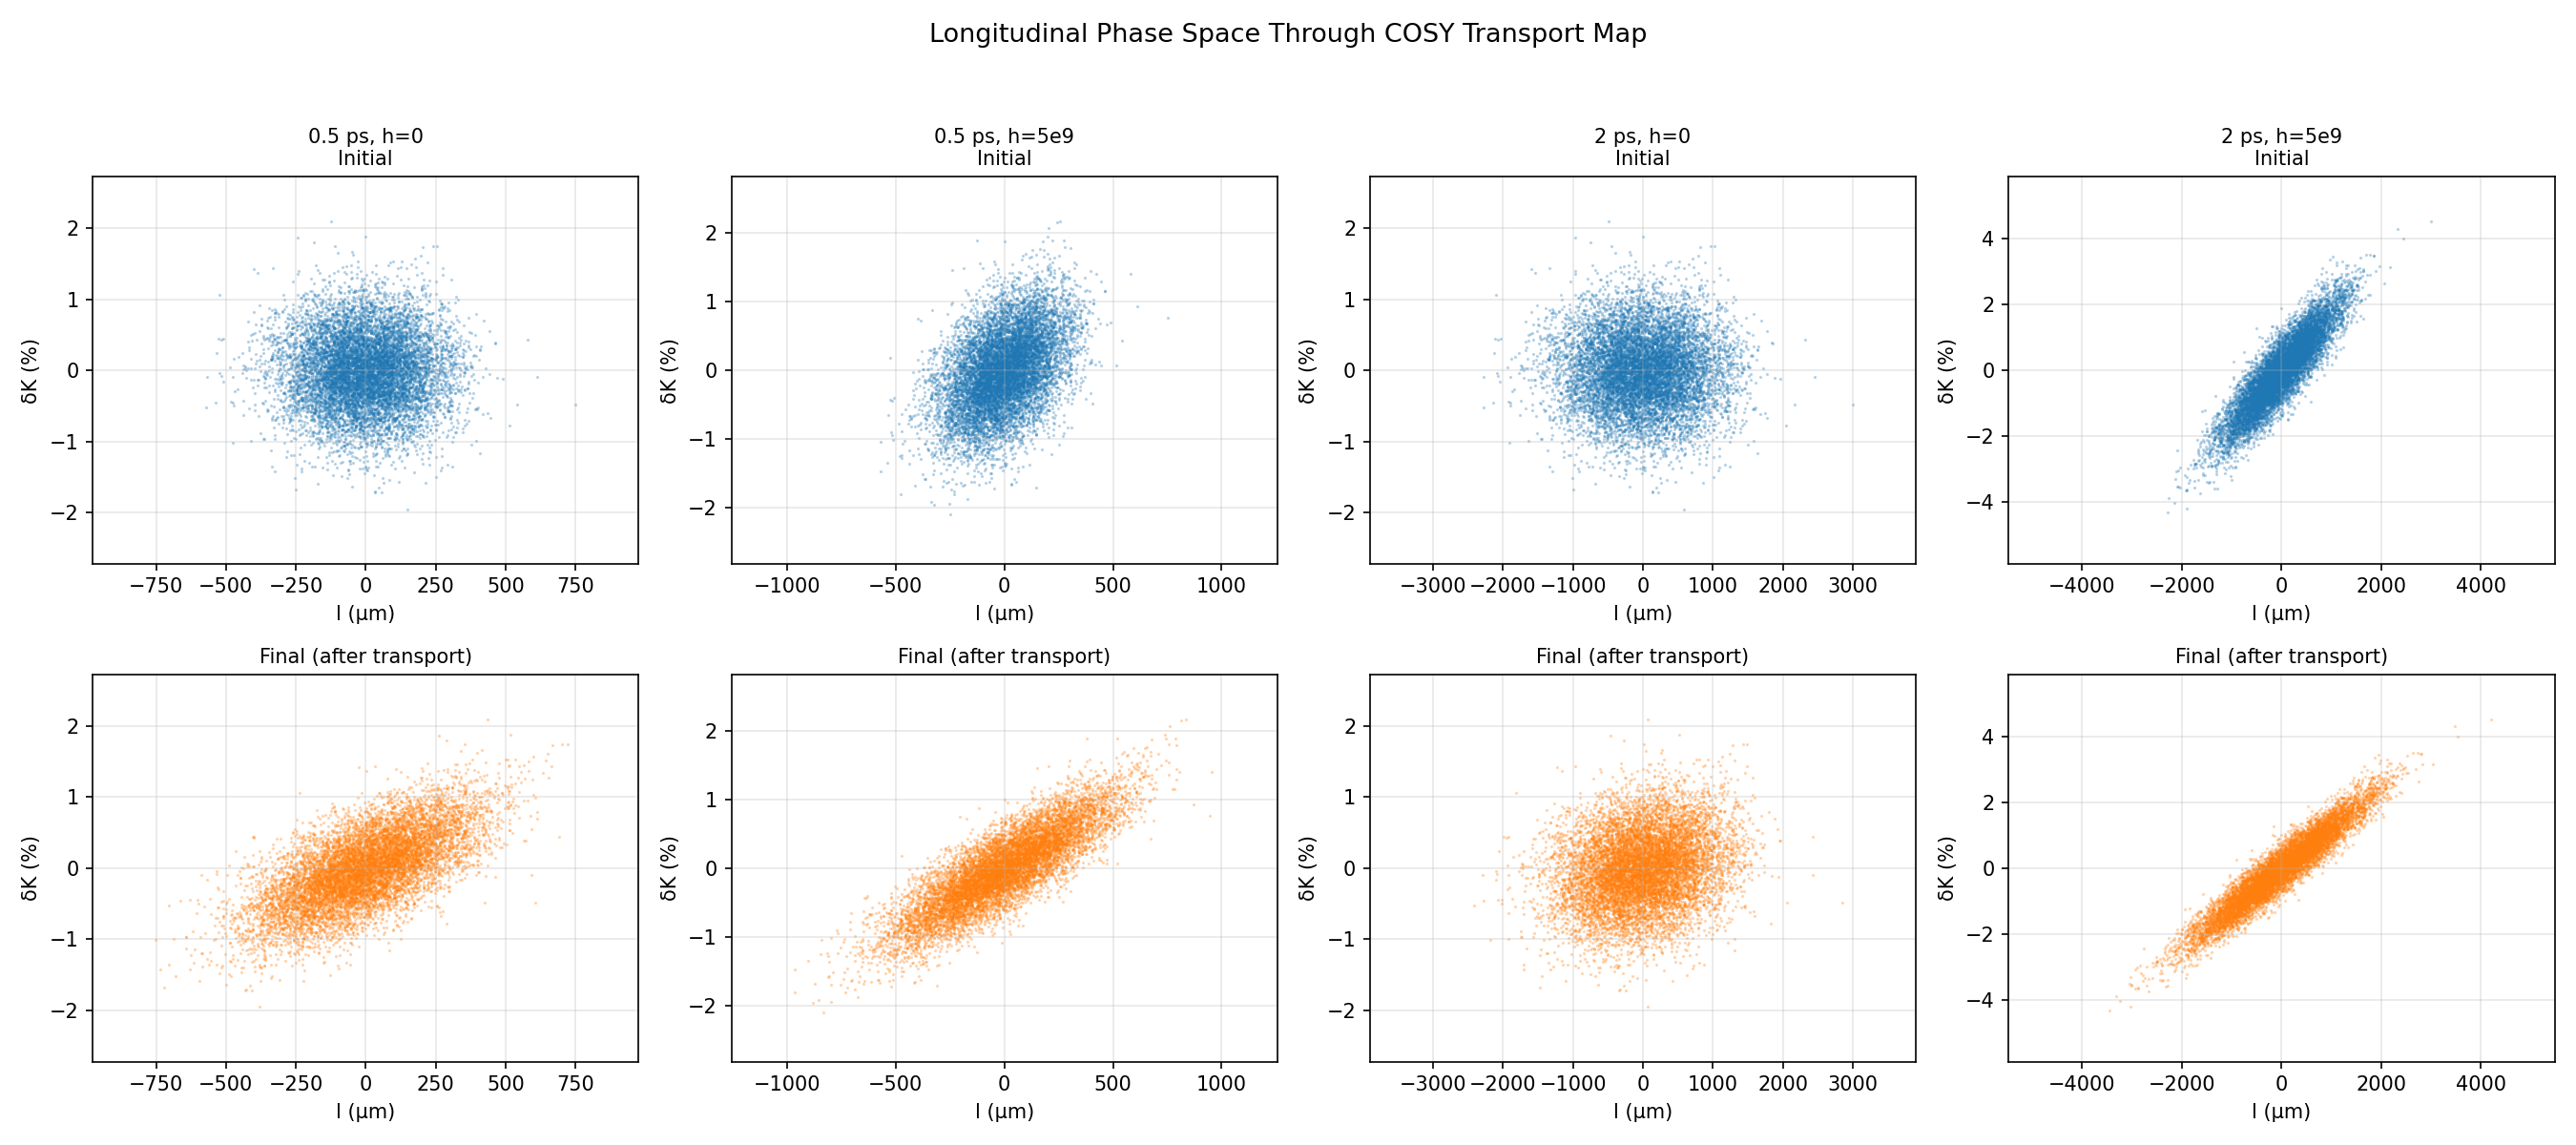
\includegraphics[width=\textwidth]{results/W9/W9_longitudinal_phase_space}
  \caption{Longitudinal phase space ($l$ vs $\delta$) before (top) and
    after (bottom) transport through the COSY map.  The 0.5\,ps
    distributions broaden visibly in $l$; the 2\,ps distributions are
    largely unchanged.  Energy spread is preserved in all cases.}
  \label{fig:phase-space}
\end{figure}

\begin{figure}[p]
  \centering
  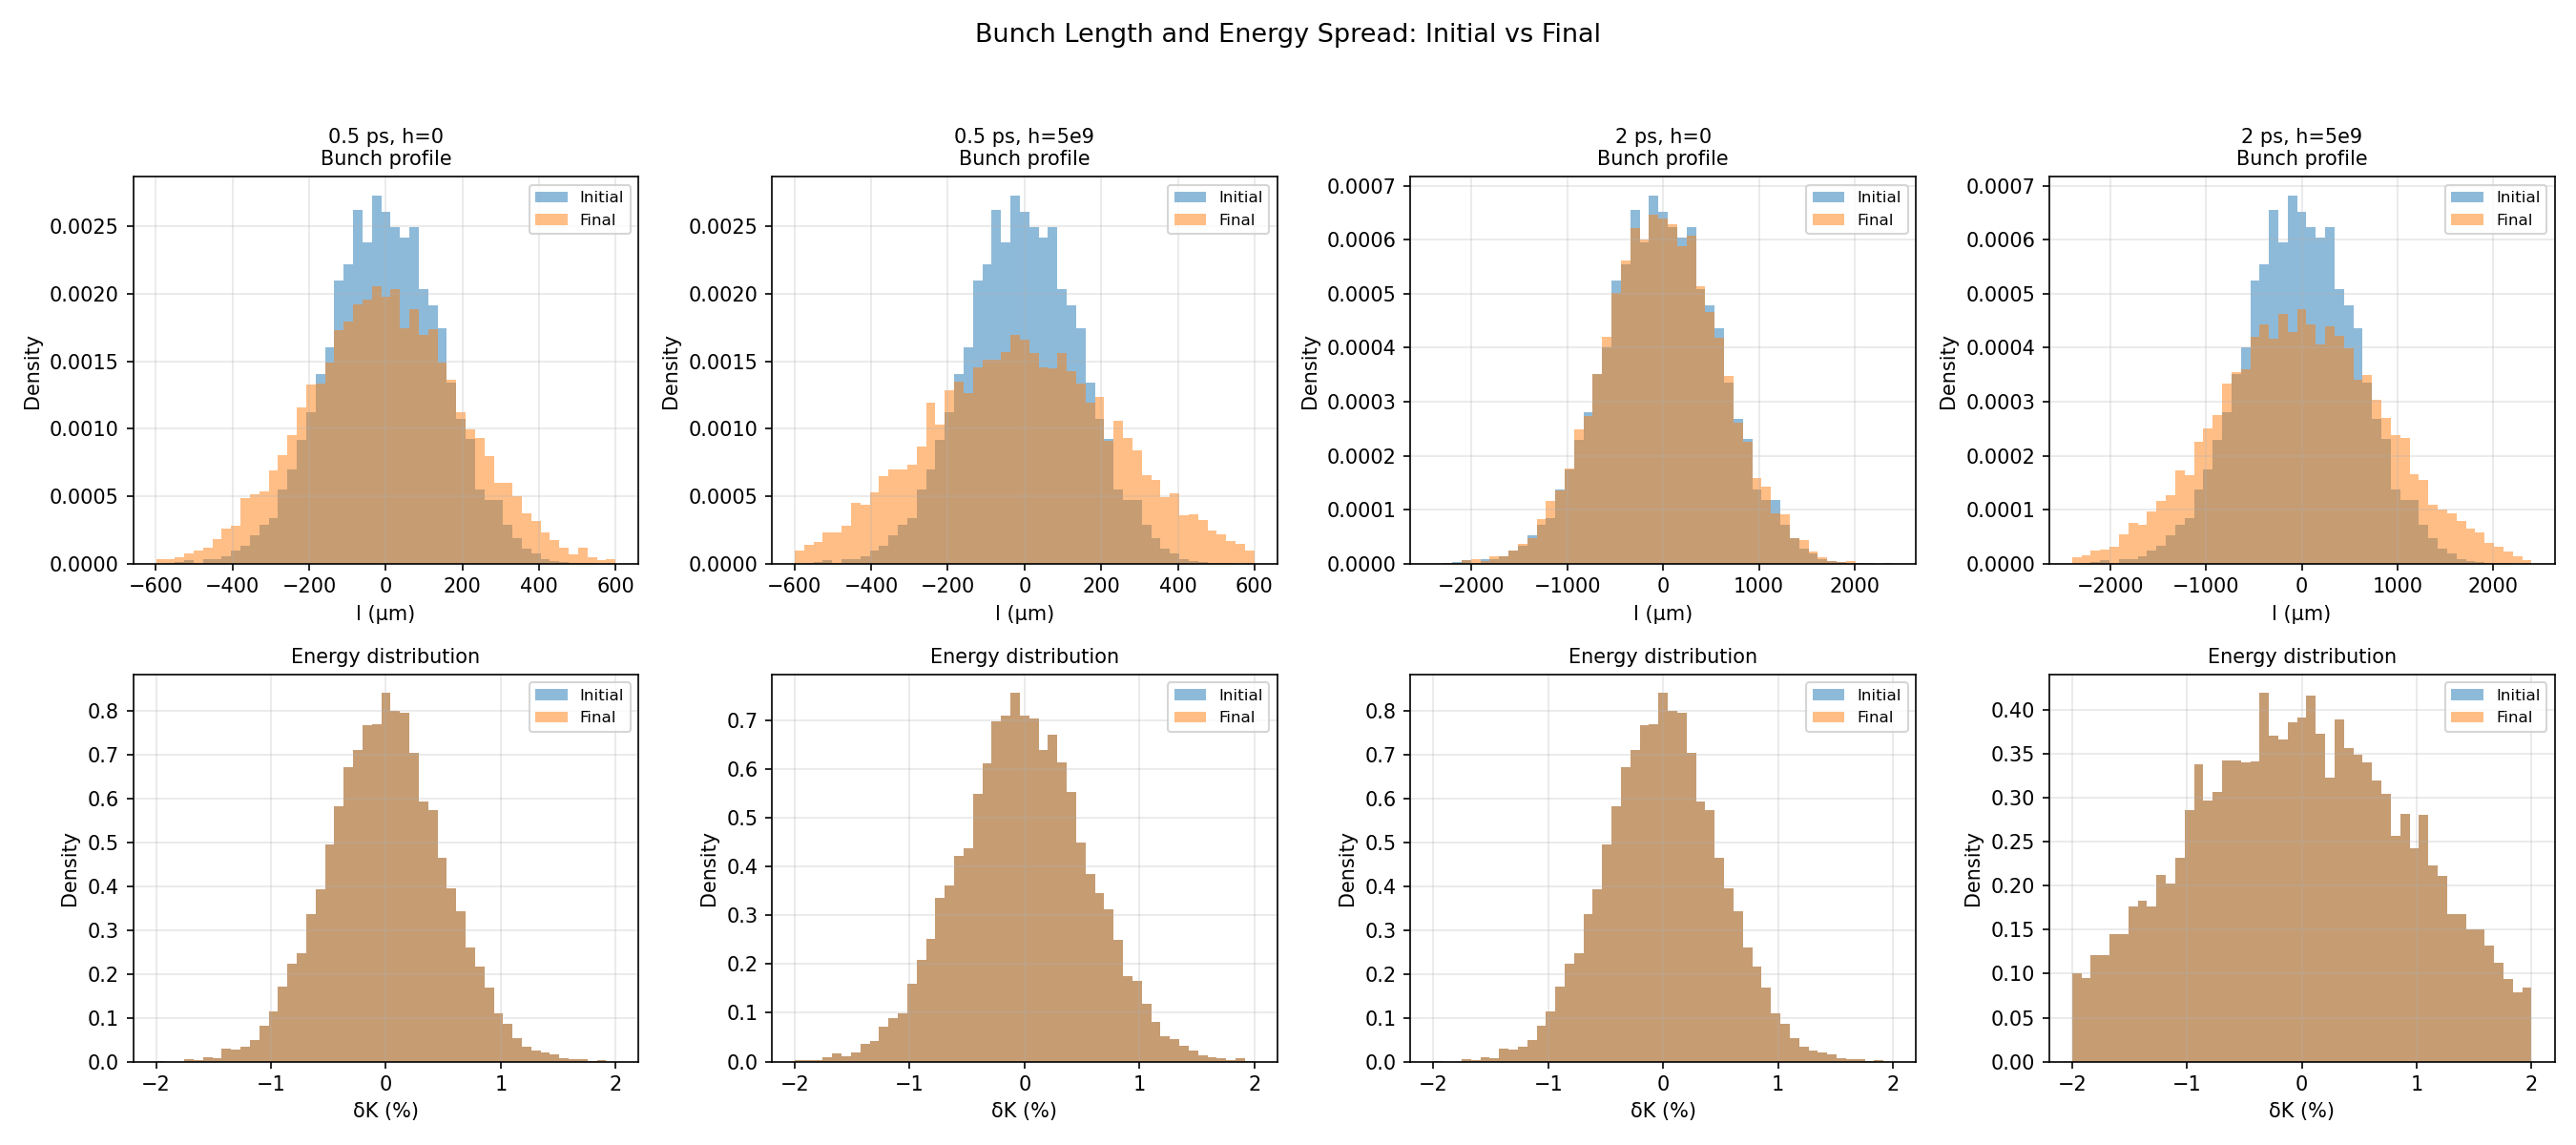
\includegraphics[width=\textwidth]{results/W9/W9_bunch_histograms}
  \caption{Bunch length (top) and energy distribution (bottom)
    histograms: initial (blue) vs final (orange).  Energy distributions
    overlap exactly; bunch profiles broaden for 0.5\,ps due to chromatic
    path-length spread.}
  \label{fig:histograms}
\end{figure}

\begin{figure}[p]
  \centering
  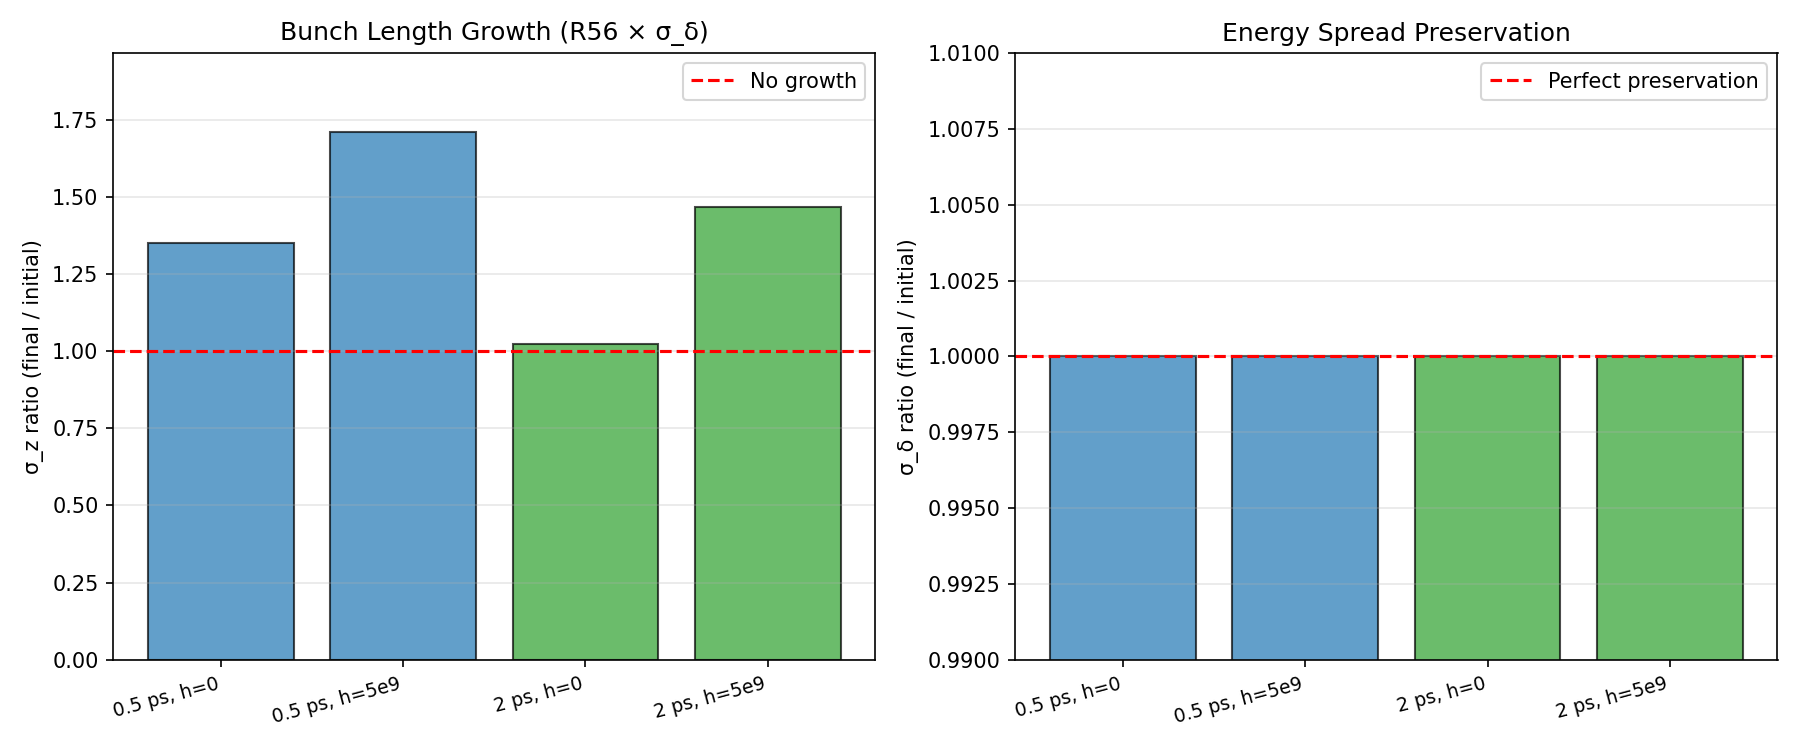
\includegraphics[width=0.85\textwidth]{results/W9/W9_preservation_ratios}
  \caption{Left: bunch length growth ratio
    $\sigma_z^\text{out}/\sigma_z^\text{in}$.  Right: energy spread
    preservation (ratio = 1.0000 for all scenarios).}
  \label{fig:ratios}
\end{figure}

\begin{figure}[p]
  \centering
  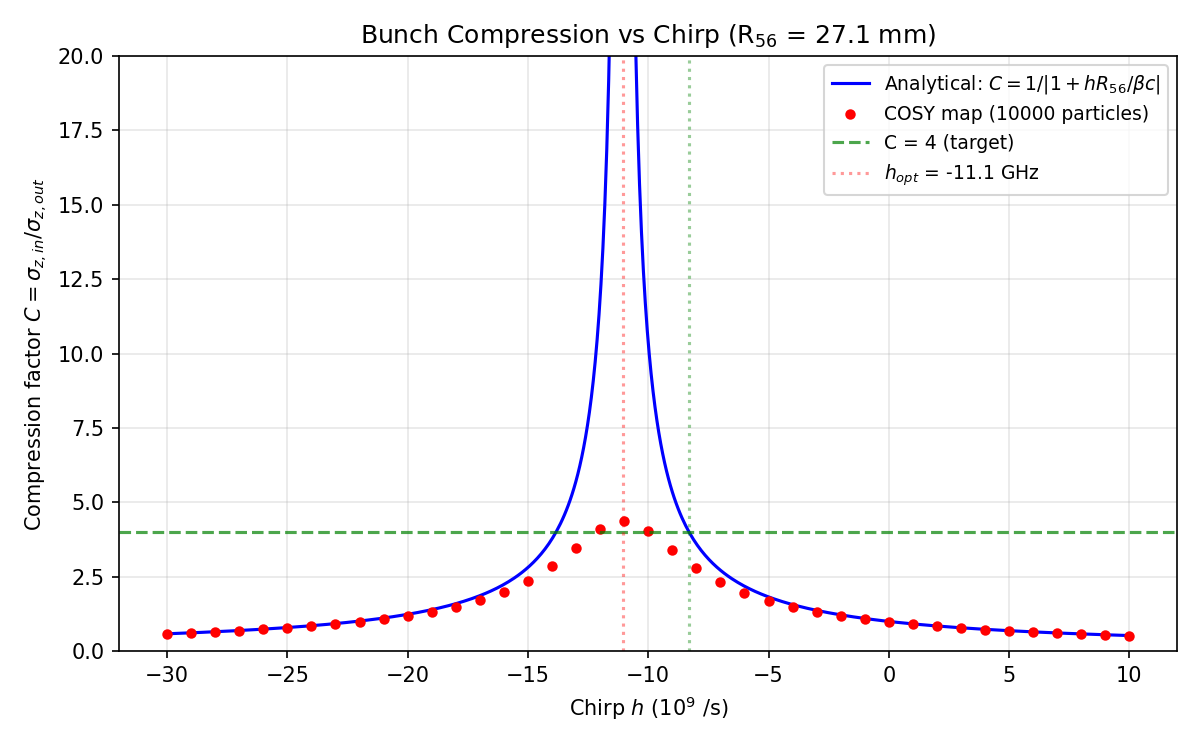
\includegraphics[width=0.85\textwidth]{results/W12/W12_compression_vs_chirp}
  \caption{Compression factor vs chirp rate.  Blue line: analytical
    $C = 1/|1 + hR_{56}/\beta c|$.  Red circles: COSY map propagation.
    Green dashed: $C = 4$ target.}
  \label{fig:compression}
\end{figure}

\begin{figure}[p]
  \centering
  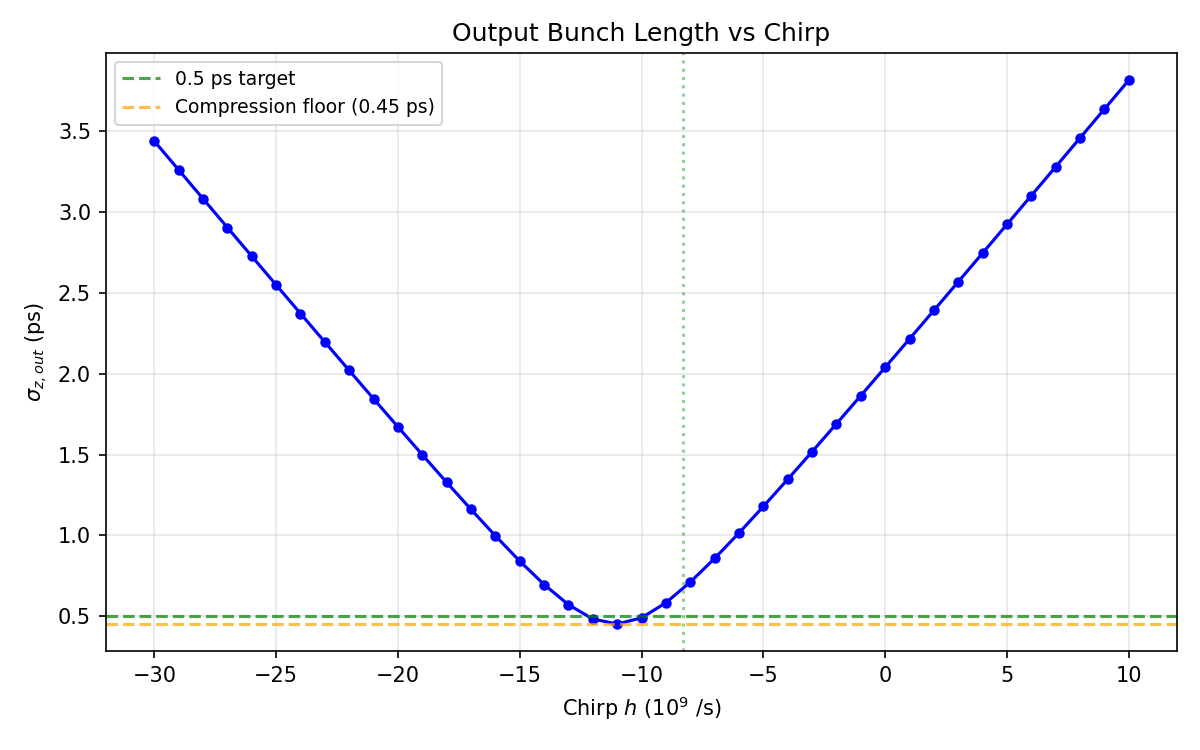
\includegraphics[width=0.85\textwidth]{results/W12/W12_sigma_z_vs_chirp}
  \caption{Output bunch length vs chirp rate.  The compression floor
    (orange dashed, \SI{0.45}{ps}) prevents reaching \SI{0.5}{ps}
    (green dashed) at practical chirp values.}
  \label{fig:sigma-z}
\end{figure}

\begin{figure}[p]
  \centering
  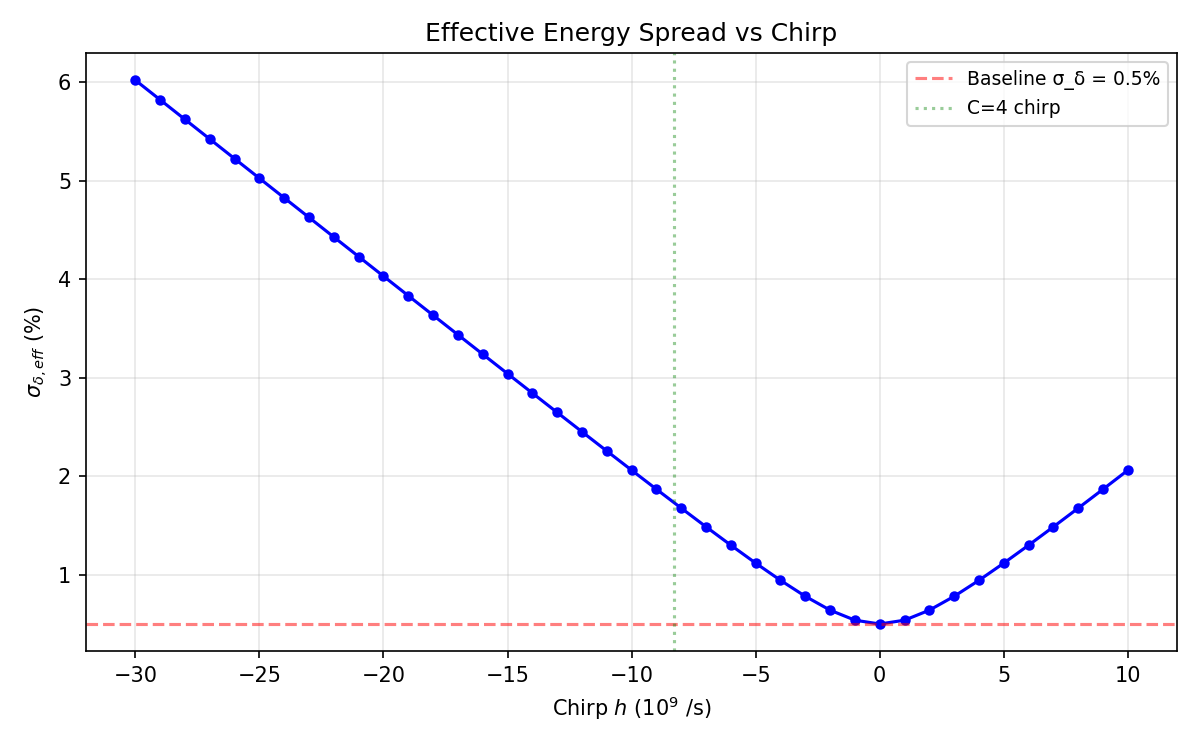
\includegraphics[width=0.85\textwidth]{results/W12/W12_sigma_delta_vs_chirp}
  \caption{Effective energy spread vs chirp rate.  At $C = 4$ chirp,
    $\sigma_{\delta,\text{eff}} \approx 1.7\%$.}
  \label{fig:sigma-delta}
\end{figure}

\begin{figure}[p]
  \centering
  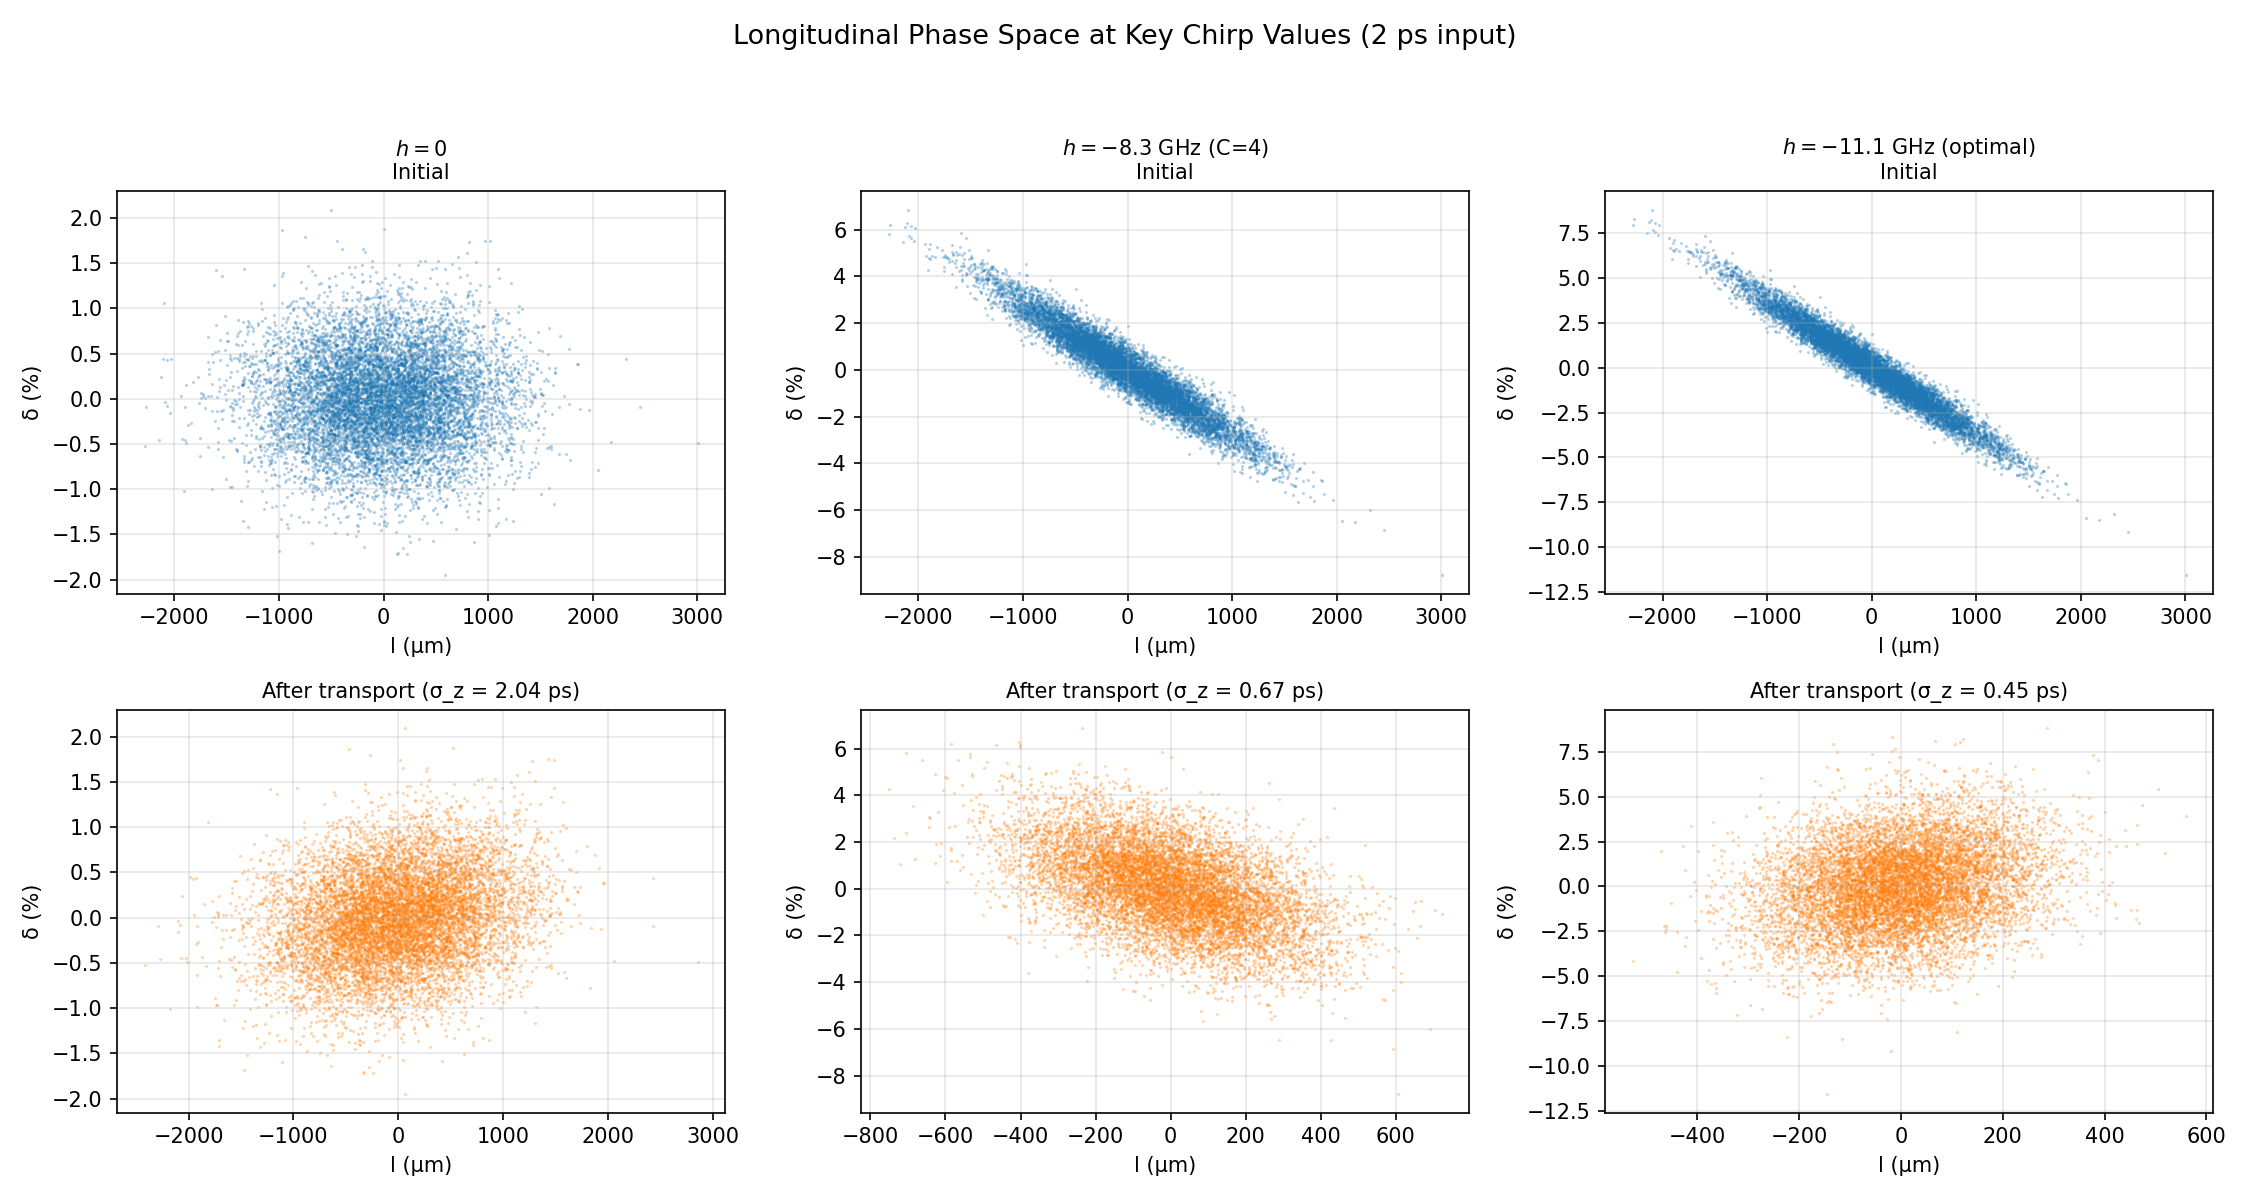
\includegraphics[width=\textwidth]{results/W12/W12_phase_space_key_chirps}
  \caption{Longitudinal phase space before (top) and after (bottom)
    transport at three chirp values.  At $h_\text{opt}$: maximum
    compression to the floor.}
  \label{fig:phase-space-chirps}
\end{figure}

\begin{figure}[p]
  \centering
  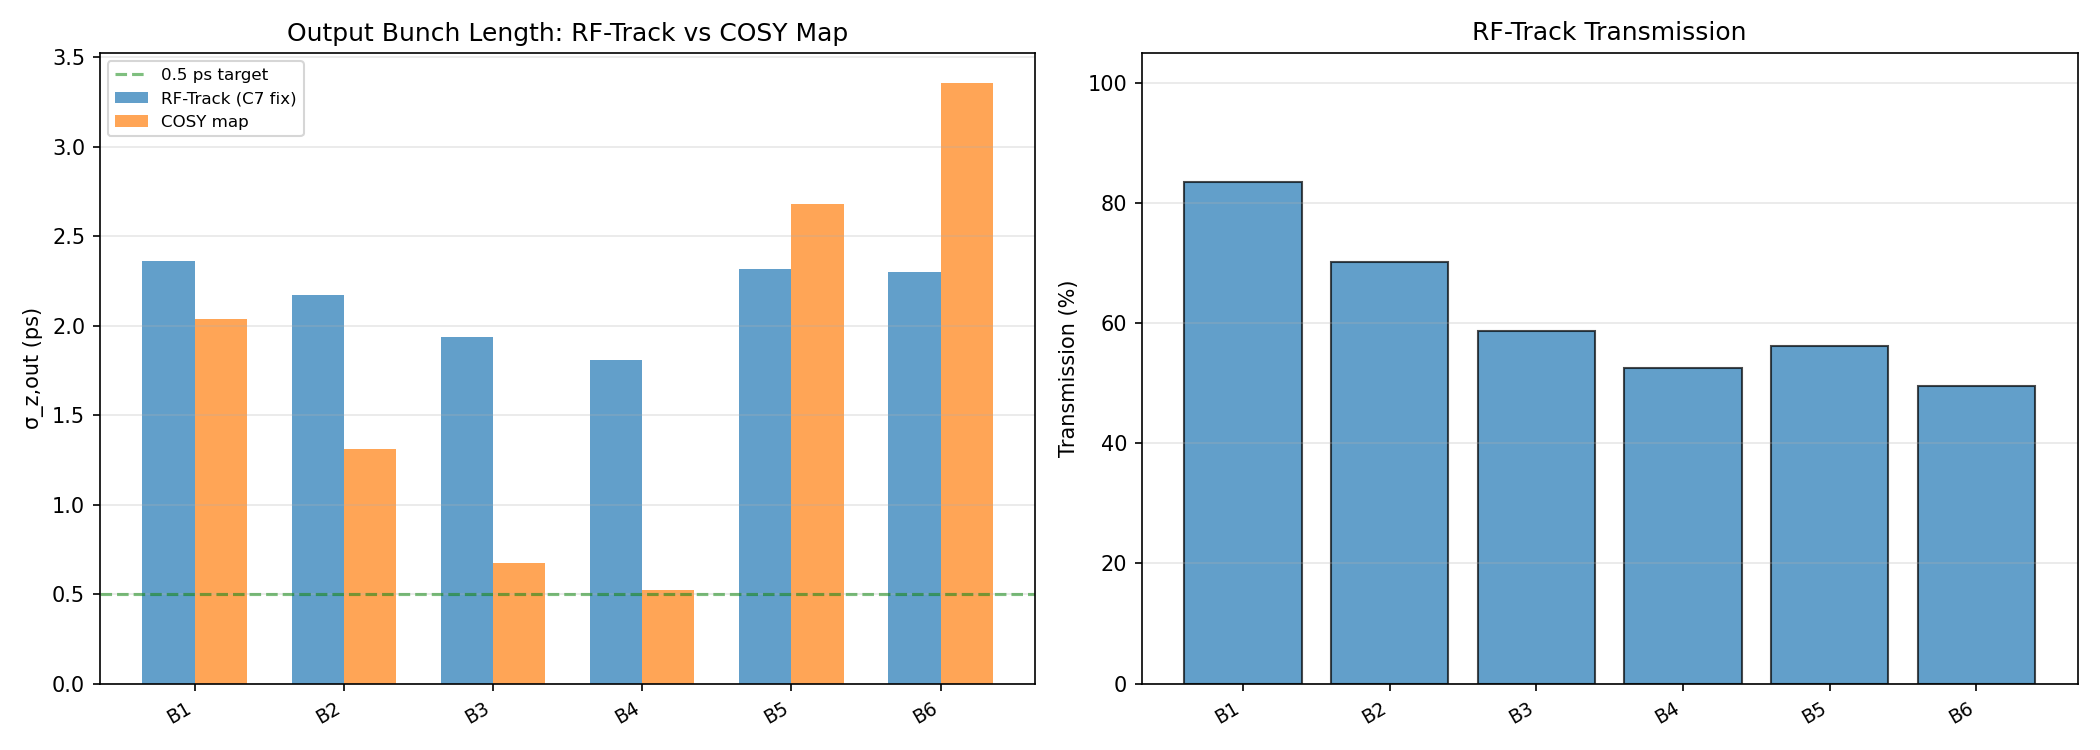
\includegraphics[width=\textwidth]{results/W12/W12_rftrack_comparison}
  \caption{Left: output bunch length from RF-Track (blue) vs COSY map
    (orange) for 6 compression scenarios.  Right: RF-Track transmission.
    The disagreement grows with chirp (B3--B4) due to aperture losses
    and nonlinear effects.}
  \label{fig:rftrack}
\end{figure}


\begin{thebibliography}{9}
\bibitem{weinberg2025}
  M.~Weinberg, A.~Fisher, and R.~Li,
  ``Design of the UH Mark V Free Electron Laser,''
  arXiv:2510.14061v1, Table~I.

\bibitem{Ferrario2010}
  M.~Ferrario \textit{et al.},
  ``Experimental Demonstration of Emittance Compensation with
  Velocity Bunching,''
  Phys.\ Rev.\ Lett.\ \textbf{104}, 054801 (2010).

\bibitem{DiMitri2012}
  S.~Di~Mitri \textit{et al.},
  ``Coherent synchrotron radiation and microbunching in bunch
  compressors and free-electron lasers,''
  Phys.\ Rev.\ ST Accel.\ Beams \textbf{15}, 020701 (2012).

\bibitem{Tono2019}
  K.~Tono, T.~Hara, M.~Yabashi, and H.~Tanaka,
  ``Multiple-beamline operation of SACLA,''
  J.\ Synchrotron Rad.\ \textbf{26}, 595--602 (2019).

\bibitem{Snedden2024}
  E.~W.~Snedden \textit{et al.},
  ``Specification and design for full energy beam exploitation of the
  compact linear accelerator for research and applications,''
  Phys.\ Rev.\ Accel.\ Beams \textbf{27}, 041602 (2024).

\bibitem{lcls-faq}
  SLAC National Accelerator Laboratory,
  ``LCLS Machine FAQ,''
  \url{https://lcls.slac.stanford.edu/machine/faq}.
\end{thebibliography}

\end{document}
